\documentclass[../thesis.tex]{subfiles}
\begin{document}
\section{Applied Integrated Lifetimes}

\subsection{CBP Host Thickness}

\begin{figure}[ht]
\centering
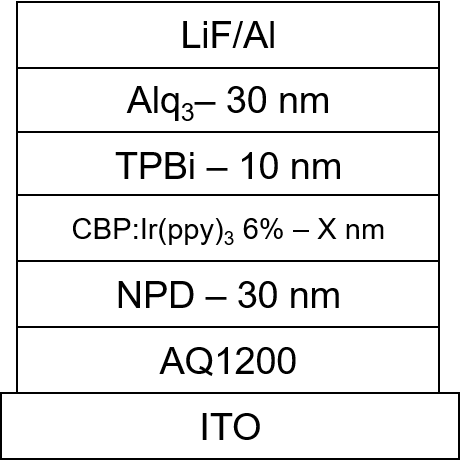
\includegraphics[scale=.25]{lifetimeApplications/architecture}
\caption{Device architecture, featuring EML thicknesses of X=10,20, and 30 nm}
\label{fig:architecture}
\end{figure}

\begin{figure}[ht]
\centering
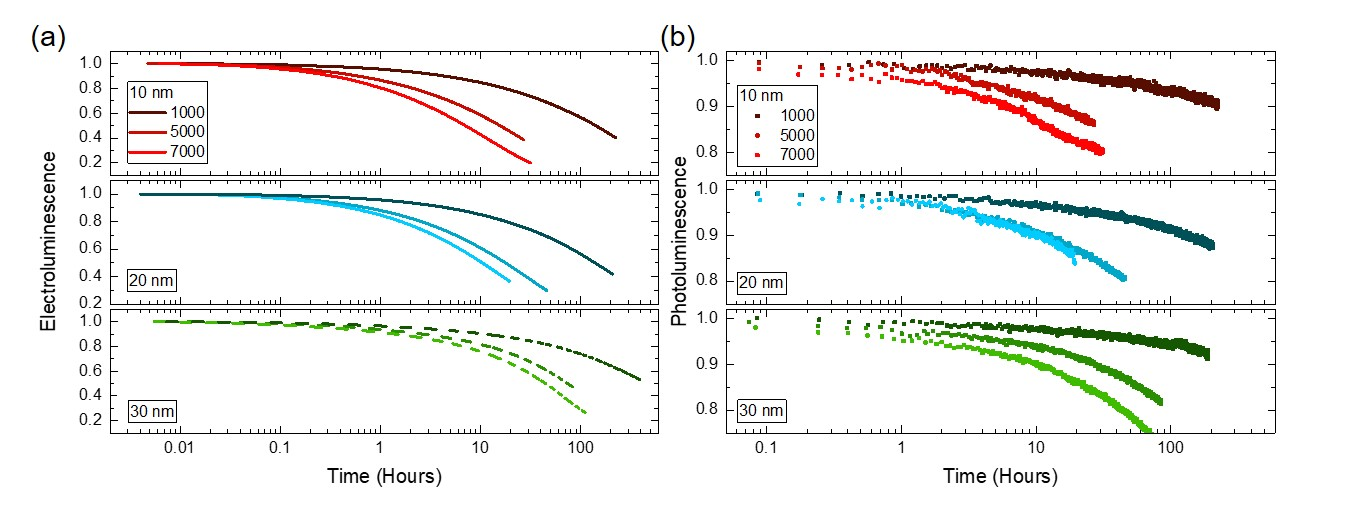
\includegraphics[scale=.25]{lifetimeApplications/elpl}
\caption{Device decay curves for multiple values of the initial luminance as a function of emissive layer thickness.  Loss in (a) electroluminescence (EL) and (b) photoluminescence (PL) are shown and decrease monotonically with increasing luminance.  For devices with a 10-nm-thick emissive layer, initial luminance values are 1000 $cd/m^2$, 5000 $cd/m^2$, and 7000 $cd/m^2$.  For devices with a 20-nm- or 30-nm-thick emissive layer, initial luminance values are 1000 $cd/m^2$, 5000 $cd/m^2$, and 7100 $cd/m^2$. }
\label{fig:elpl}
\end{figure}

\begin{figure}[ht]
\centering
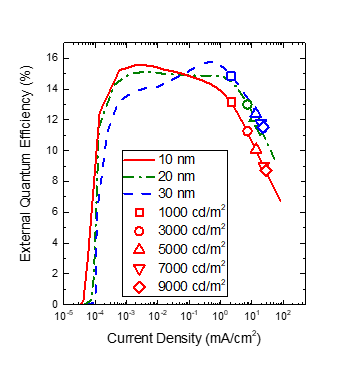
\includegraphics[scale=.25]{lifetimeApplications/eqe}
\caption{External Quantum Efficienct ($\eta_{EQE}$) for the three architectures.  Operational points for lifetime are shown in symbols.}
\label{fig:eqe}
\end{figure}

\begin{figure}[ht]
\centering
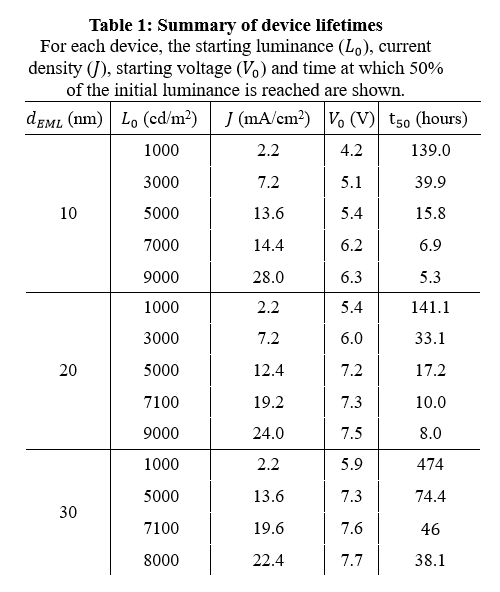
\includegraphics[scale=.25]{lifetimeApplications/lifetime_table}
\label{fig:lifetime_table}
\end{figure}

\begin{figure}[ht]
\centering
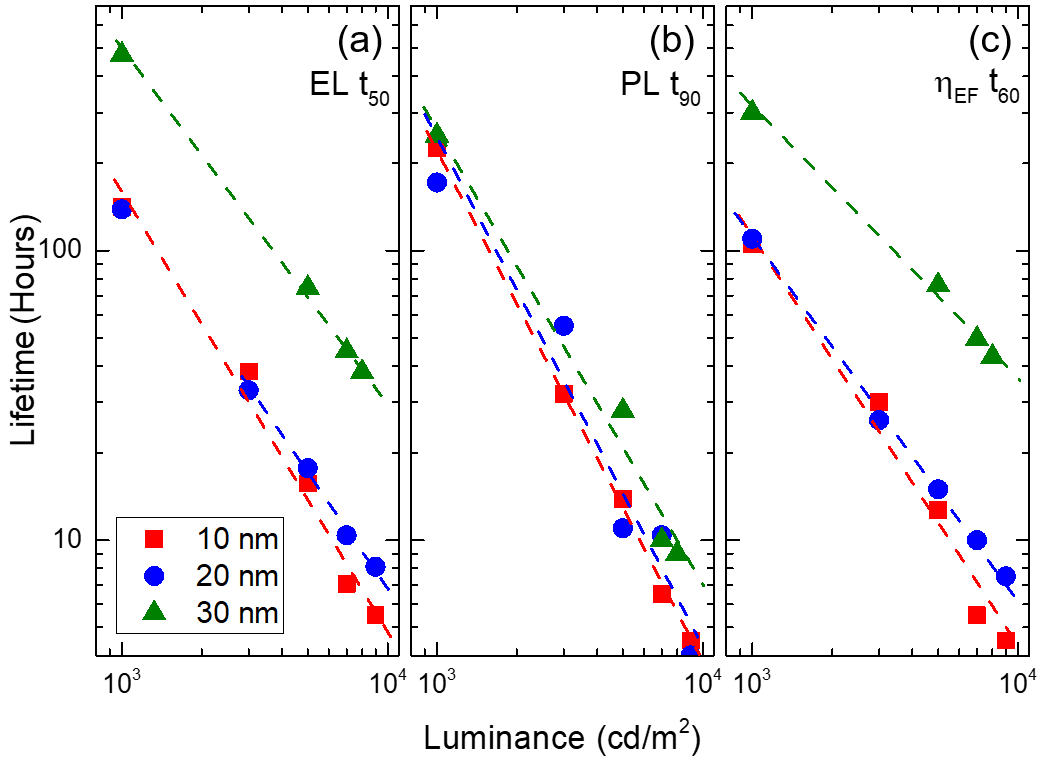
\includegraphics[scale=.25]{lifetimeApplications/tx_components}
\caption{Extracted lifetimes for all 3 architecures as a function of luminance.}
\label{fig:tx_components}
\end{figure}

\subsection{MEML Luminance Scaling}


\subsection{Dow Cohost}



\ifcsdef{mainfile}{}{\bibliography{../thesis}}
\end{document}
